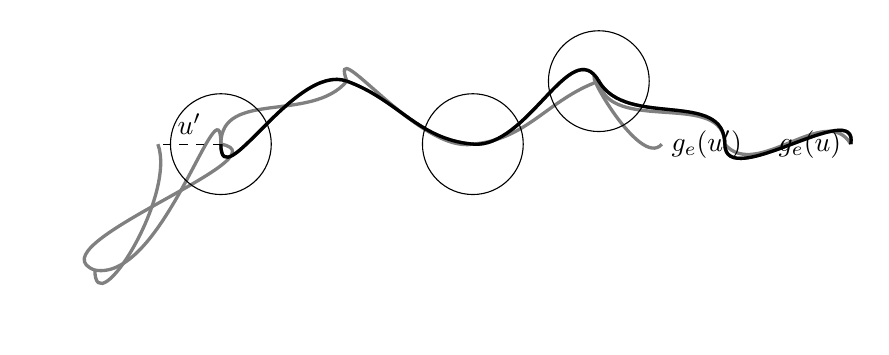
\begin{tikzpicture}[scale=0.8]
%original part of the walk in grey
\draw[color=gray,very thick] (-2,-3) to[out=-10,in=90] (0,-1) to[out=-90,in=160] (2,0) to[out=-20,in=175] (4,-1) to[out=-5,in=120] (6,0) to[out=-60,in=90] (8,-1) to[out=-90,in=80] (10,-1);
\draw[color=gray,very thick] (-2,-3) to[out=160,in=-10] (0,-1) to[out=90,in=230] (2,0) to[out=110,in=-170] (4,-1) to[out=5,in=200] (6,0) to[out=-80,in=90] (8,-1);
\draw[color=gray,very thick] (-2,-3) to[out=-90,in=-70] (-1,-1);
\draw[color=gray,very thick] (6,0) to[out=130,in=-130] (7,-1);
\draw[color=gray,very thick] (8,-1) to[out=-50,in=120] (10,-1);

%modified part of the walk in black
\draw[very thick] (0,-1) to[out=-90,in=160] (2,0);
\draw[very thick] (2,0) to[out=-20,in=175] (4,-1);
\draw[very thick] (4,-1) to[out=-5,in=120] (6,0);
\draw[very thick] (6,0) to[out=-60,in=90] (8,-1);
\draw[very thick] (8,-1) to[out=-90,in=80] (10,-1);

%splitted point u
\draw[dashed] (0,-1)--(-1,-1);
\node[above] at (-0.5,-1) {$u'$};
%splitted point g_e(u')
\node[right] at (7,-1) {$g_{e}(u')$};
%splitted point g_e(u)
\node[right] at (8.7,-1) {$g_{e}(u)$};

\draw (0,-1) circle[radius=0.8];
\draw (4,-1) circle[radius=0.8];
\draw (6,0) circle[radius=0.8];

\end{tikzpicture}